% Options for packages loaded elsewhere
\PassOptionsToPackage{unicode}{hyperref}
\PassOptionsToPackage{hyphens}{url}
\PassOptionsToPackage{dvipsnames,svgnames,x11names}{xcolor}
%
\documentclass[
  letterpaper,
  DIV=11,
  numbers=noendperiod]{scrartcl}

\usepackage{amsmath,amssymb}
\usepackage{lmodern}
\usepackage{iftex}
\ifPDFTeX
  \usepackage[T1]{fontenc}
  \usepackage[utf8]{inputenc}
  \usepackage{textcomp} % provide euro and other symbols
\else % if luatex or xetex
  \usepackage{unicode-math}
  \defaultfontfeatures{Scale=MatchLowercase}
  \defaultfontfeatures[\rmfamily]{Ligatures=TeX,Scale=1}
\fi
% Use upquote if available, for straight quotes in verbatim environments
\IfFileExists{upquote.sty}{\usepackage{upquote}}{}
\IfFileExists{microtype.sty}{% use microtype if available
  \usepackage[]{microtype}
  \UseMicrotypeSet[protrusion]{basicmath} % disable protrusion for tt fonts
}{}
\makeatletter
\@ifundefined{KOMAClassName}{% if non-KOMA class
  \IfFileExists{parskip.sty}{%
    \usepackage{parskip}
  }{% else
    \setlength{\parindent}{0pt}
    \setlength{\parskip}{6pt plus 2pt minus 1pt}}
}{% if KOMA class
  \KOMAoptions{parskip=half}}
\makeatother
\usepackage{xcolor}
\setlength{\emergencystretch}{3em} % prevent overfull lines
\setcounter{secnumdepth}{-\maxdimen} % remove section numbering
% Make \paragraph and \subparagraph free-standing
\ifx\paragraph\undefined\else
  \let\oldparagraph\paragraph
  \renewcommand{\paragraph}[1]{\oldparagraph{#1}\mbox{}}
\fi
\ifx\subparagraph\undefined\else
  \let\oldsubparagraph\subparagraph
  \renewcommand{\subparagraph}[1]{\oldsubparagraph{#1}\mbox{}}
\fi


\providecommand{\tightlist}{%
  \setlength{\itemsep}{0pt}\setlength{\parskip}{0pt}}\usepackage{longtable,booktabs,array}
\usepackage{calc} % for calculating minipage widths
% Correct order of tables after \paragraph or \subparagraph
\usepackage{etoolbox}
\makeatletter
\patchcmd\longtable{\par}{\if@noskipsec\mbox{}\fi\par}{}{}
\makeatother
% Allow footnotes in longtable head/foot
\IfFileExists{footnotehyper.sty}{\usepackage{footnotehyper}}{\usepackage{footnote}}
\makesavenoteenv{longtable}
\usepackage{graphicx}
\makeatletter
\def\maxwidth{\ifdim\Gin@nat@width>\linewidth\linewidth\else\Gin@nat@width\fi}
\def\maxheight{\ifdim\Gin@nat@height>\textheight\textheight\else\Gin@nat@height\fi}
\makeatother
% Scale images if necessary, so that they will not overflow the page
% margins by default, and it is still possible to overwrite the defaults
% using explicit options in \includegraphics[width, height, ...]{}
\setkeys{Gin}{width=\maxwidth,height=\maxheight,keepaspectratio}
% Set default figure placement to htbp
\makeatletter
\def\fps@figure{htbp}
\makeatother

\KOMAoption{captions}{tableheading}
\makeatletter
\@ifpackageloaded{tcolorbox}{}{\usepackage[many]{tcolorbox}}
\@ifpackageloaded{fontawesome5}{}{\usepackage{fontawesome5}}
\definecolor{quarto-callout-color}{HTML}{909090}
\definecolor{quarto-callout-note-color}{HTML}{0758E5}
\definecolor{quarto-callout-important-color}{HTML}{CC1914}
\definecolor{quarto-callout-warning-color}{HTML}{EB9113}
\definecolor{quarto-callout-tip-color}{HTML}{00A047}
\definecolor{quarto-callout-caution-color}{HTML}{FC5300}
\definecolor{quarto-callout-color-frame}{HTML}{acacac}
\definecolor{quarto-callout-note-color-frame}{HTML}{4582ec}
\definecolor{quarto-callout-important-color-frame}{HTML}{d9534f}
\definecolor{quarto-callout-warning-color-frame}{HTML}{f0ad4e}
\definecolor{quarto-callout-tip-color-frame}{HTML}{02b875}
\definecolor{quarto-callout-caution-color-frame}{HTML}{fd7e14}
\makeatother
\makeatletter
\makeatother
\makeatletter
\makeatother
\makeatletter
\@ifpackageloaded{caption}{}{\usepackage{caption}}
\AtBeginDocument{%
\ifdefined\contentsname
  \renewcommand*\contentsname{Table of contents}
\else
  \newcommand\contentsname{Table of contents}
\fi
\ifdefined\listfigurename
  \renewcommand*\listfigurename{List of Figures}
\else
  \newcommand\listfigurename{List of Figures}
\fi
\ifdefined\listtablename
  \renewcommand*\listtablename{List of Tables}
\else
  \newcommand\listtablename{List of Tables}
\fi
\ifdefined\figurename
  \renewcommand*\figurename{Figure}
\else
  \newcommand\figurename{Figure}
\fi
\ifdefined\tablename
  \renewcommand*\tablename{Table}
\else
  \newcommand\tablename{Table}
\fi
}
\@ifpackageloaded{float}{}{\usepackage{float}}
\floatstyle{ruled}
\@ifundefined{c@chapter}{\newfloat{codelisting}{h}{lop}}{\newfloat{codelisting}{h}{lop}[chapter]}
\floatname{codelisting}{Listing}
\newcommand*\listoflistings{\listof{codelisting}{List of Listings}}
\makeatother
\makeatletter
\@ifpackageloaded{caption}{}{\usepackage{caption}}
\@ifpackageloaded{subcaption}{}{\usepackage{subcaption}}
\makeatother
\makeatletter
\@ifpackageloaded{tcolorbox}{}{\usepackage[many]{tcolorbox}}
\makeatother
\makeatletter
\@ifundefined{shadecolor}{\definecolor{shadecolor}{rgb}{.97, .97, .97}}
\makeatother
\makeatletter
\makeatother
\ifLuaTeX
  \usepackage{selnolig}  % disable illegal ligatures
\fi
\IfFileExists{bookmark.sty}{\usepackage{bookmark}}{\usepackage{hyperref}}
\IfFileExists{xurl.sty}{\usepackage{xurl}}{} % add URL line breaks if available
\urlstyle{same} % disable monospaced font for URLs
\hypersetup{
  pdftitle={NLP-QuAL Results},
  colorlinks=true,
  linkcolor={blue},
  filecolor={Maroon},
  citecolor={Blue},
  urlcolor={Blue},
  pdfcreator={LaTeX via pandoc}}

\title{NLP-QuAL Results}
\author{}
\date{}

\begin{document}
\maketitle
\ifdefined\Shaded\renewenvironment{Shaded}{\begin{tcolorbox}[borderline west={3pt}{0pt}{shadecolor}, enhanced, interior hidden, sharp corners, breakable, frame hidden, boxrule=0pt]}{\end{tcolorbox}}\fi

\renewcommand*\contentsname{Table of contents}
{
\hypersetup{linkcolor=}
\setcounter{tocdepth}{3}
\tableofcontents
}
\hypertarget{qual-score}{%
\subsection{QuAL Score}\label{qual-score}}

As a review, the QuAL score aims to assess the quality of written
feedback for medical trainees. It has been validated in a GME context.
It ranges from 0 (lowest quality) to 6 (highest quality). It is the sum
of three subscores:

\begin{itemize}
\tightlist
\item
  Q1 - Does the rater provide sufficient evidence about resident
  performance? (Rated on a three-point scale: 0-no comment at all, 1-no,
  but comment present, 2-somewhat, 3-yes/full description)
\item
  Q2 - Suggestion - Does the rater provide a suggestion for improvement?
  (0-no/1-yes)
\item
  Q3 - Connection - Is the rater's suggestion linked to the behavior
  described? (0-no/1-yes)
\end{itemize}

\hypertarget{data-descriptives-and-demographics}{%
\subsection{Data Descriptives and
Demographics}\label{data-descriptives-and-demographics}}

We analyzed 2500 evaluations, with 1250 from Site 1 (McMaster) and 1250
from Site 2 (Saskatchewan).

For each evaluation, the QuAL score was rated by two separate raters.
Each sub-score (Q1, Q2, and Q3) was rated and then summed to get the
final QuAL score. Discrepancies were broken by members of the study team
(who?)

The average QuAL score was 2.6408, with standard deviation 1.275, median
3.0

Descriptive statistics for the subscores and QuAL Score were:

\hypertarget{tbl-descrips}{}
\begin{longtable}[]{@{}lllll@{}}
\caption{\label{tbl-descrips}Descriptive Statistics for
Subscores/QuAL}\tabularnewline
\toprule()
& Q1 & Q2 & Q3 & QUAL \\
\midrule()
\endfirsthead
\toprule()
& Q1 & Q2 & Q3 & QUAL \\
\midrule()
\endhead
count & 2500.000000 & 2500.000000 & 2500.000000 & 2500.000000 \\
mean & 2.277200 & 0.193600 & 0.170000 & 2.640800 \\
std & 0.860149 & 0.395198 & 0.375708 & 1.275157 \\
50\% & 3.000000 & 0.000000 & 0.000000 & 3.000000 \\
\bottomrule()
\end{longtable}

\hypertarget{score-distributions}{%
\subsubsection{Score Distributions}\label{score-distributions}}

\hypertarget{subscores}{%
\paragraph{Subscores}\label{subscores}}

\hypertarget{tbl-distsubscore}{}
\begin{longtable}[]{@{}lllllll@{}}
\caption{\label{tbl-distsubscore}Subscore Rating
Counts/Frequencies}\tabularnewline
\toprule()
& Q1 & & Q2 & & Q3 & \\
\midrule()
\endfirsthead
\toprule()
& Q1 & & Q2 & & Q3 & \\
\midrule()
\endhead
& Count & Percent of Total & Count & Percent of Total & Count & Percent
of Total \\
0 & 105 & 4.20 & 2016.0 & 80.64 & 2075.0 & 83.0 \\
1 & 359 & 14.36 & 484.0 & 19.36 & 425.0 & 17.0 \\
2 & 774 & 30.96 & NaN & NaN & NaN & NaN \\
3 & 1262 & 50.48 & NaN & NaN & NaN & NaN \\
\bottomrule()
\end{longtable}

The distribution for the subscores is plotted below:

\begin{figure}

\begin{minipage}[t]{0.33\linewidth}

{\centering 

\raisebox{-\height}{

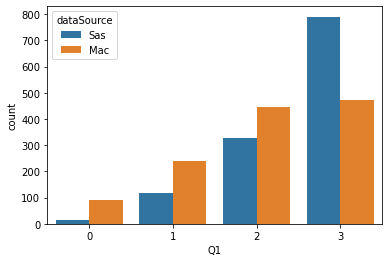
\includegraphics{results_lite_files/figure-pdf/fig-distsubscores-output-1.png}

}

}

\subcaption{\label{fig-distsubscores-1}Q1}
\end{minipage}%
%
\begin{minipage}[t]{0.33\linewidth}

{\centering 

\raisebox{-\height}{

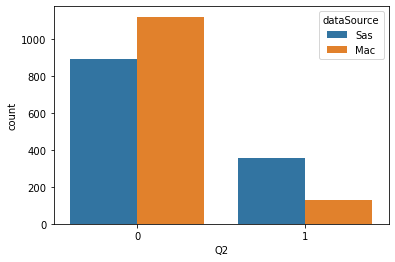
\includegraphics{results_lite_files/figure-pdf/fig-distsubscores-output-2.png}

}

}

\subcaption{\label{fig-distsubscores-2}Q2}
\end{minipage}%
%
\begin{minipage}[t]{0.33\linewidth}

{\centering 

\raisebox{-\height}{

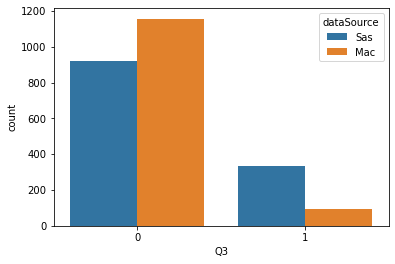
\includegraphics{results_lite_files/figure-pdf/fig-distsubscores-output-3.png}

}

}

\subcaption{\label{fig-distsubscores-3}Q3}
\end{minipage}%

\caption{\label{fig-distsubscores}Distribution of QuAL Subscores}

\end{figure}

Evaluations tended to score highly (\textgreater{} 2) on Q1, but poorly
(80\% 0 and 83\% 0, respectively) on Q2 and Q3. There were large
differences in scores between the two sites.

\hypertarget{qual-score-1}{%
\paragraph{QuAL Score}\label{qual-score-1}}

The table below shows the raw counts and percentages associated with
each level of the rated QuAL score.

\hypertarget{tbl-distqual}{}
\begin{longtable}[]{@{}lll@{}}
\caption{\label{tbl-distqual}QuAL Rating
Counts/Frequencies}\tabularnewline
\toprule()
& Count & Percent of Total \\
\midrule()
\endfirsthead
\toprule()
& Count & Percent of Total \\
\midrule()
\endhead
0 & 100 & 4.00 \\
1 & 338 & 13.52 \\
2 & 685 & 27.40 \\
3 & 957 & 38.28 \\
4 & 77 & 3.08 \\
5 & 343 & 13.72 \\
\bottomrule()
\end{longtable}

The distribution of the QuAL score is plotted below:

\begin{figure}

{\centering 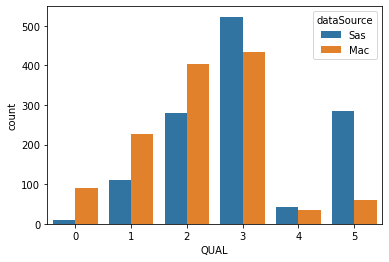
\includegraphics{results_lite_files/figure-pdf/fig-distqual-output-1.png}

}

\caption{\label{fig-distqual}Distribution of QuAL Subscores}

\end{figure}

This table shows the counts/frequencies for each possible combination of
subscores. For each possible final QuAL score, the table shows the
combination fo subscores most likely to generate that QuAL score.

\hypertarget{tbl-qualcounts}{}
\begin{longtable}[]{@{}llllll@{}}
\caption{\label{tbl-qualcounts}Subscore Combinations/Counts for each
QuAL Score}\tabularnewline
\toprule()
& & & & Count & Percent of Total \\
\midrule()
\endfirsthead
\toprule()
& & & & Count & Percent of Total \\
\midrule()
\endhead
QUAL & Q1 & Q2 & Q3 & & \\
0 & 0 & 0 & 0 & 100 & 4.00 \\
1 & 0 & 1 & 0 & 5 & 0.20 \\
& 1 & 0 & 0 & 333 & 13.32 \\
2 & 1 & 0 & 1 & 1 & 0.04 \\
& & 1 & 0 & 21 & 0.84 \\
& 2 & 0 & 0 & 663 & 26.52 \\
3 & 1 & 1 & 1 & 4 & 0.16 \\
& 2 & 0 & 1 & 2 & 0.08 \\
& & 1 & 0 & 41 & 1.64 \\
& 3 & 0 & 0 & 910 & 36.40 \\
4 & 2 & 1 & 1 & 68 & 2.72 \\
& 3 & 0 & 1 & 7 & 0.28 \\
& & 1 & 0 & 2 & 0.08 \\
5 & 3 & 1 & 1 & 343 & 13.72 \\
\bottomrule()
\end{longtable}

This table yields some interesting insights. The QuAL score subscores
are dependent on one another. Based on the structure of the subscores,
it follows that if the evaluation is not detailed enough (Q1 \(\leq\)
2), it's unlikely to contain a suggestion for improvement (Q1 = 0), and
there can be no linking between behavior and improvement (Q3 = 0). The
table backs this up, with the vast majority of Q2 and Q3 rated as zero
if Q1 \(\leq\) 2. If the evaluation is highly detailed (Q3 = 3), then
naturally it is more likely to have a suggestion for improvement (Q2 =
1), and based on the table, it's also likely to link the suggestion to
the behavior (Q3 = 1). Q3 is essentially redundant; Q3 is discrepant
from Q2 in only 3.1\% of all evaluations.

This means that the QuAL score can be reduced to three primary outcomes:

\begin{itemize}
\tightlist
\item
  Q1 \(\leq\) 2 - low detail, very unlikely (\textless10\%) to contain
  suggestion for improvement
\item
  Q1 = 3; Q2 and Q3 = 0 - high detail, no suggestion for improvement
\item
  Q1 = 3; Q2 and Q3 = 1 - high detail, with suggestion for improvement,
  extremely likely to have connection between behavior/suggestion
\end{itemize}

These three scenarios fit 2,349/2,500 = 94\% of evaluations. This
provides an opportunity to condense the QuAL score from 6 levels (0-5)
to 3. Although the remainder of the results below do \emph{not} condense
the QuAL score, this could be a good way to boost accuracy results in a
way that does not compromise the integrity of the score itself.

\hypertarget{interrater-reliability}{%
\subsubsection{Interrater Reliability}\label{interrater-reliability}}

This table shows the percent agreement for the QUAL score and each
subscore

\hypertarget{tbl-percentmatch}{}
\begin{longtable}[]{@{}lllllllll@{}}
\caption{\label{tbl-percentmatch}Interrater Agreement Counts and
Frequencies}\tabularnewline
\toprule()
& Q1Match & & Q2Match & & Q3Match & & QUALMatch & \\
\midrule()
\endfirsthead
\toprule()
& Q1Match & & Q2Match & & Q3Match & & QUALMatch & \\
\midrule()
\endhead
& Count & Percent of Total & Count & Percent of Total & Count & Percent
of Total & Count & Percent of Total \\
False & 1059 & 42.36 & 188 & 7.52 & 606 & 24.24 & 1426 & 57.04 \\
True & 1441 & 57.64 & 2312 & 92.48 & 1894 & 75.76 & 1074 & 42.96 \\
\bottomrule()
\end{longtable}

\hypertarget{tbl-kappa}{}
\begin{longtable}[]{@{}ll@{}}
\caption{\label{tbl-kappa}Cohen's Kappas}\tabularnewline
\toprule()
& Cohen's Kappa \\
\midrule()
\endfirsthead
\toprule()
& Cohen's Kappa \\
\midrule()
\endhead
Q1 & 0.387601 \\
Q2 & 0.751249 \\
Q3 & 0.351520 \\
QuAL & 0.317628 \\
\bottomrule()
\end{longtable}

Cohen's Kappas were calculated and are presented above. There was fair
agreement for all scores except for Q2, which had substantial agreement.
This was before any tiebreaking/discrepancy correction.

\hypertarget{other-demographics-and-descriptive-statistics}{%
\subsubsection{Other Demographics and Descriptive
Statistics}\label{other-demographics-and-descriptive-statistics}}

These may or may not be relevant.

\hypertarget{tbl-gender}{}
\begin{longtable}[]{@{}lllll@{}}
\caption{\label{tbl-gender}Reported Genders (actually sexes) of
Residents and Faculty}\tabularnewline
\toprule()
& GenderRes & & GenderFac & \\
\midrule()
\endfirsthead
\toprule()
& GenderRes & & GenderFac & \\
\midrule()
\endhead
& Count & Percent of Total & Count & Percent of Total \\
Female & 1037.0 & 41.48 & 877 & 35.08 \\
Male & 1463.0 & 58.52 & 1447 & 57.88 \\
Unknown & NaN & NaN & 176 & 7.04 \\
\bottomrule()
\end{longtable}

ObserverType stratifies the evaluator by role.

\hypertarget{tbl-observertype}{}
\begin{longtable}[]{@{}lll@{}}
\caption{\label{tbl-observertype}Evaluator Types}\tabularnewline
\toprule()
& ObserverType & \\
\midrule()
\endfirsthead
\toprule()
& ObserverType & \\
\midrule()
\endhead
& Count & Percent of Total \\
clinical supervisor & 1200 & 48.0 \\
faculty & 1165 & 46.6 \\
resident & 135 & 5.4 \\
\bottomrule()
\end{longtable}

Only one of the two sites reports PGY levels for their trainees on their
evaluations.

\hypertarget{tbl-pgy}{}
\begin{longtable}[]{@{}ll@{}}
\caption{\label{tbl-pgy}Reported PGY years of learners}\tabularnewline
\toprule()
& PGY \\
\midrule()
\endfirsthead
\toprule()
& PGY \\
\midrule()
\endhead
Unknown & 1251 \\
2 & 510 \\
1 & 456 \\
3 & 157 \\
4 & 117 \\
5 & 9 \\
\bottomrule()
\end{longtable}

\hypertarget{model-performance}{%
\subsection{Model Performance}\label{model-performance}}

\hypertarget{metrics}{%
\subsubsection{Metrics}\label{metrics}}

Models were assessed using the following performance metrics:

\begin{itemize}
\tightlist
\item
  \emph{Balanced Accuracy} - The weighted average of accuracies for each
  possible class (rating). In situations where the data is imbalanced,
  including this one, accuracy can be falsely inflated if the model
  over-biases against the rare classes. Balanced accuracy compensates
  for this and provides a more valid assessment of model performance in
  the real world. It is the most important metric evaluated.
\item
  \emph{Accuracy} - The percentage of time the model made the correct
  guess about the rating
\item
  \emph{Top 2 Accuracy} - The percentage of time the model's first guess
  \textbf{or} second guess was correct. Only applies to targets with
  \(\geq\) 3 levels (Q1 and overall QuAL)
\item
  \emph{Top 3 Accuracy} - Same as above but includes first, second, or
  third guess.
\item
  \emph{Mean absolute error (MAE)} - Average discrepancy between the
  model's guess and the true rating. Useful for Q1 and QuAL.
\item
  \emph{ROC AUC Score} - Area under the receiver operating curve. Common
  metric reported in ML literature. Subject to inflation if classes are
  imbalanced. Only well-defined for two-class targets (Q2 and Q3).
\item
  \emph{Precision} - Positive predictive value, the chance that a
  ``positive'' prediction (usually defined as the outcome of interest,
  in this case \textbf{lower} quality) is actually correct. Best defined
  for two-class targets, but averages can be taken for multi-class
  targets (Q1 and QuAL).
\item
  \emph{Recall} - Sensitivity
\item
  \emph{F1} - The geometric mean of precision and recall, often reported
  in the ML literature.
\item
  \emph{Confusion Matrix} - A \emph{n\_classes} by \emph{n\_classes}
  matrix, where the \(i,j\)th entry is the number of items with true
  rating \(i\) and predicted rating \(j\). A perfect classifier would
  produce a confusion matrix non-zero only on the diagonal. The
  confusion matrix shows you which ratings the model is struggling with.
\item
  \emph{Support} - Not a metric, \emph{per se}, but the number of items
  in the test set which received the given rating.
\end{itemize}

\hypertarget{q1}{%
\subsubsection{Q1}\label{q1}}

Q1 assessed the level of evidence about the learner's performance
provided in the evaluation. Specifically, Q1 asked, ``Does the rater
provide sufficient evidence about resident performance?'' It was rated
on a three-point scale: 0-no comment at all, 1-no, but comment present,
2-somewhat, 3-yes/full description.

The table below shows the model performance metrics for Q1.

\hypertarget{tbl-q1metrics}{}
\begin{longtable}[]{@{}ll@{}}
\caption{\label{tbl-q1metrics}Q1 Metrics}\tabularnewline
\toprule()
& Score \\
\midrule()
\endfirsthead
\toprule()
& Score \\
\midrule()
\endhead
balanced\_accuracy & 0.590736 \\
accuracy & 0.624000 \\
top\_2\_acc & 0.880000 \\
top\_3\_acc & 0.973333 \\
precision & 0.620417 \\
recall & 0.590736 \\
f1 & 0.598159 \\
\bottomrule()
\end{longtable}

Overall, model performance for Q1 is relatively weak when considered
from an absolute accuracy standpoint, getting on average 59\% of
predictions correct. However, as Q1 has four possible ratings (0-3),
random guessing would be correct only 25\% of the time, so our model
performs 2.36 times better than random. Looking at the Top 2 Accuracy,
we see the model contains the true rating within its top-2 predictions
88\% of the time, which further demonstrates that the model is ``on the
right track.''

Exploring performance by class level and visualizing the confusion
matrix, we can begin to see the reasons for high/low performance:

\hypertarget{tbl-q1byrating}{}
\begin{longtable}[]{@{}lll@{}}
\caption{\label{tbl-q1byrating}Q1 Performance by Rating}\tabularnewline
\toprule()
& F1 Score & Support \\
\midrule()
\endfirsthead
\toprule()
& F1 Score & Support \\
\midrule()
\endhead
Q1 Rating & & \\
0 & 0.727273 & 25.0 \\
1 & 0.400000 & 49.0 \\
2 & 0.500000 & 113.0 \\
3 & 0.765363 & 188.0 \\
\bottomrule()
\end{longtable}

\begin{figure}

{\centering 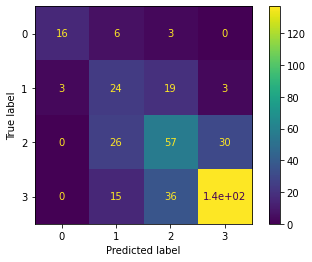
\includegraphics{results_lite_files/figure-pdf/fig-q1conf-output-1.png}

}

\caption{\label{fig-q1conf}Q1 Confusion Matrix}

\end{figure}

The model performs best at the extremes, the Q1 = 0 and Q1 = 3 ratings
perform well, but when Q1 = 1 and Q1 = 2, the model has trouble
differentiating the ``nuances'' at this level. This is to be expected,
as the human raters struggled to differentiate between these levels as
well. The table below shows the percent of human rater agreement for Q1
stratified by Q1 rating:

\hypertarget{tbl-q1humanmatch}{}
\begin{longtable}[]{@{}ll@{}}
\caption{\label{tbl-q1humanmatch}Percent Human Match by Q1
Rating}\tabularnewline
\toprule()
& Percent Human Match \\
\midrule()
\endfirsthead
\toprule()
& Percent Human Match \\
\midrule()
\endhead
Q1 & \\
0 & 97.142857 \\
1 & 84.679666 \\
2 & 40.439276 \\
3 & 57.210777 \\
\bottomrule()
\end{longtable}

\hypertarget{q2}{%
\subsubsection{Q2}\label{q2}}

Q2 assessed whether or not the evaluator provided a suggestion for
improvement in the written evaluation. It asked, ``Does the rater
provide a suggestion for improvement? (0-no/1-yes)''

\begin{tcolorbox}[enhanced jigsaw, titlerule=0mm, left=2mm, colbacktitle=quarto-callout-note-color!10!white, breakable, colback=white, rightrule=.15mm, arc=.35mm, coltitle=black, opacityback=0, opacitybacktitle=0.6, bottomtitle=1mm, toptitle=1mm, bottomrule=.15mm, colframe=quarto-callout-note-color-frame, leftrule=.75mm, title=\textcolor{quarto-callout-note-color}{\faInfo}\hspace{0.5em}{Note}, toprule=.15mm]
Because it is more important to identify low-quality feedback, when the
model was trained, the ratings were inverted. That is, the ``positive''
(thing that needed to be identified) was switched to Q2 = \textbf{0}.
\end{tcolorbox}

The table below shows the model performance metrics for Q3.

\hypertarget{tbl-q2metrics}{}
\begin{longtable}[]{@{}ll@{}}
\caption{\label{tbl-q2metrics}Q2 Metrics}\tabularnewline
\toprule()
& Score \\
\midrule()
\endfirsthead
\toprule()
& Score \\
\midrule()
\endhead
balanced\_accuracy & 0.775220 \\
accuracy & 0.834667 \\
precision & 0.923611 \\
recall & 0.869281 \\
f1 & 0.895623 \\
\bottomrule()
\end{longtable}

Q2 was the highest performing model, as it represented the simplest
question - simply, was there a suggestion or not. It was better at
predicting if there was \emph{not} a suggestion. It had 92\% sensitivity
detecting failure to provide a suggestion, with a PPV of 86.9\%.

\hypertarget{q3}{%
\subsubsection{Q3}\label{q3}}

Q3 assessed if the evalutor connected the learner's behavior with the
suggestion for improvement. Specifically, it asked, ``Is the rater's
suggestion linked to the behavior described? (0-no/1-yes)''

\begin{tcolorbox}[enhanced jigsaw, titlerule=0mm, left=2mm, colbacktitle=quarto-callout-note-color!10!white, breakable, colback=white, rightrule=.15mm, arc=.35mm, coltitle=black, opacityback=0, opacitybacktitle=0.6, bottomtitle=1mm, toptitle=1mm, bottomrule=.15mm, colframe=quarto-callout-note-color-frame, leftrule=.75mm, title=\textcolor{quarto-callout-note-color}{\faInfo}\hspace{0.5em}{Note}, toprule=.15mm]
Because it is more important to identify low-quality feedback, when the
model was trained, the ratings were inverted. That is, the ``positive''
(thing that needed to be identified) was switched to Q3 = \textbf{0}.
\end{tcolorbox}

The table below shows the model performance metrics for Q3.

\hypertarget{tbl-q3metrics}{}
\begin{longtable}[]{@{}ll@{}}
\caption{\label{tbl-q3metrics}Q3 Metrics}\tabularnewline
\toprule()
& Score \\
\midrule()
\endfirsthead
\toprule()
& Score \\
\midrule()
\endhead
balanced\_accuracy & 0.764813 \\
accuracy & 0.845333 \\
precision & 0.933333 \\
recall & 0.880503 \\
f1 & 0.906149 \\
\bottomrule()
\end{longtable}

Q3 performed as well or better than Q2. It had a 93\% sensitivity for
failure to connect action to suggestion and a PPV of 88\%. Q2 and Q3 are
nearly redundant (discrepant only 3\% of the time), as show in
Table~\ref{tbl-qualcounts}, so it makes sense that Q3 is a
high-performer.

\hypertarget{qual}{%
\subsubsection{QuAL}\label{qual}}

The table below shows the model performance metrics for the overall QuAL
score.

\hypertarget{tbl-qualmetrics}{}
\begin{longtable}[]{@{}ll@{}}
\caption{\label{tbl-qualmetrics}QuAL Metrics}\tabularnewline
\toprule()
& Score \\
\midrule()
\endfirsthead
\toprule()
& Score \\
\midrule()
\endhead
balanced\_accuracy & 0.438582 \\
accuracy & 0.469333 \\
top\_2\_acc & 0.749333 \\
top\_3\_acc & 0.890667 \\
mae & 0.722667 \\
precision & 0.439958 \\
recall & 0.438582 \\
f1 & 0.435110 \\
\bottomrule()
\end{longtable}

The model performs fair overall. A random guess gives an accuracy of
0.167, our accuracy is 0.438. Top-2 accuracy is significantly improved,
at 0.749. Mean absolute error is only 0.772, meaning the model is right
(off by less than 1) more than it is wrong (off by 1 or more).

Exploring performance by class level and visualizing the confusion
matrix, we can begin to see the reasons for high/low performance:

\hypertarget{tbl-qualbyrating}{}
\begin{longtable}[]{@{}lll@{}}
\caption{\label{tbl-qualbyrating}QuAL Performance by Rating
Level}\tabularnewline
\toprule()
& F1 Score & Support \\
\midrule()
\endfirsthead
\toprule()
& F1 Score & Support \\
\midrule()
\endhead
QuAL Rating & & \\
0 & 0.711111 & 24.0 \\
1 & 0.336449 & 46.0 \\
2 & 0.336735 & 99.0 \\
3 & 0.577617 & 150.0 \\
4 & 0.071429 & 9.0 \\
5 & 0.577320 & 47.0 \\
\bottomrule()
\end{longtable}

\begin{figure}

{\centering 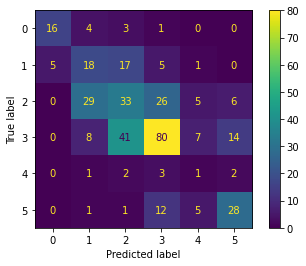
\includegraphics{results_lite_files/figure-pdf/fig-qualconf-output-1.png}

}

\caption{\label{fig-qualconf}QuAL Confusion Matrix}

\end{figure}

Once again, the model performs best at the extremes. It technically
performs worst for QuAL = 4, but there are so few actual examples rated
4 that it is essentially uninterpretable. It otherwise struggles most in
the QuAL = 1 and QuAL = 2 categories. This makes sense, as the Q1 model
above struggles most for Q1 = 1 and Q1 = 2, and based on
Table~\ref{tbl-qualcounts}, Q2/Q3 don't play much of a role until Q1 =
3. The most interesting finding here is that the model naturally assumes
the structure described in Table~\ref{tbl-qualcounts}. That is, three
``true'' ratings: Q1 \(\leq\) 2 and Q2/3 = 0 (QuAL = 0-2); Q1 = 3 and
Q2/3 = 0 (QuAL = 3); and Q1 = 3 and Q2/3 = 1 (QuAL = 5).

\hypertarget{discussion-and-next-steps}{%
\section{Discussion and Next Steps}\label{discussion-and-next-steps}}

\hypertarget{interpretation-of-accuracy}{%
\subsection{Interpretation of
Accuracy}\label{interpretation-of-accuracy}}

It is difficult to interpret the overall performance of the model. As a
number, 46\% accurracy does not sound particularly impressive, though
when you consider it is a 6-point scale, there is some leeway,
particularly given the high top-2 accuracy and relatively low mean
absolute error. Interpreting the accuracy is also difficult without
anything to compare it to. The closesest is the
\href{https://pubmed.ncbi.nlm.nih.gov/33951682/}{Otles et al paper}
(Brian George group), which demonstrated an accuracy of 0.64 on a
4-level scale. Having subscores works to our advantage, as our
performance on Q2 and Q3 is stellar, and it allows us to say that we are
predicting something new and interesting compared to prior approaches.

\hypertarget{next-steps}{%
\subsection{Next Steps}\label{next-steps}}

Overall, this analysis makes the strongest case for condensing the QuAL
score. At the very least, QuAL = 4 should be removed. Based on the
analyses above, the QuAL score seems more like a thresholded 3-level
score, rather than a 6 level score. Q1 can be condensed to two levels
(Q1 \(\leq\) 2 and Q1 = 3), and Q3 should be eliminated as it is
redundant with Q2. This will significantly increase our accuracy, at the
expense of some increased complexity in justifying why we condensed the
score. It will also better model the real-world behavior of the score.

The modeling above should be re-run with the condensed score. Deep
learning approaches should also be tried, especially for Q1.



\end{document}
